\documentclass{llncs}

\usepackage[utf8]{inputenc}

\usepackage{listings}
\usepackage{amssymb}
\usepackage{amsmath}
\usepackage{pdfpages}

\title{Five Message Handshake Project in Spin}
\titlerunning{Five Message Handshake}
\author{Alexander Steen \and Max Wisniewski}
\date{\today}
\institute{Institut f\"ur Informatik, FU Berlin}

\begin{document}

\maketitle

\begin{abstract}
The distributed algorithm for the mutual exclusion problem proposed by Suzuki and Kasami \cite{Suzuki:1985:DME:6110.214406} is checked
with the modelchecker \emph{Spin}. We present a modeling for the algorithm in Promela, the properties we want
to check for this algorithm and a short error analysis, why the second algorithm of Suzuki and Kasami does not work.
\end{abstract}



%% --------------------------------------
%%           Section I
%% --------------------------------------
\section{Introduction}

In the 1980s, Ricard and Agrawala published a distributed algorithm the solves the mutual exclusion
problem for networks of independent agents. This algorithm requires $2N-2$ message exchanges per
invocation, where $N$ is the number of agents in the network~\cite{Ricart:1981:OAM:358527.358537}.
In 1985, Sizuki and Kasami proposed a different algorithm which is supposed to solve the problem of 
mutual exclusion yet only requiring $N$ messages per invocation. A modification of this algorithm
only uses bounded counters and requires asymptoticaly $N$ messages per invocation as the number of
invocations grow.
Section~\ref{sec:prob} gives an overview of the problem and the solution proposed by Suzuki and Kasami.
The remainder of this document describes how those algorithms can be modeled in promela and
processed by the spin modelchecker.

%% --------------------------------------
%%           Section II
%% --------------------------------------
\section{Problem / Algorithm\label{sec:prob}}

The proposed algorithm is a solution for the distributed mutual exclusion problem.

Given $N$ processes that can only communicate over messages and that do not have shared memory
and a critical section we want to find a protocol such that at any time at most one process
works in the critical section.

As in the concurrent case we want this protocol to satisfy \emph{mutual exclusion}, absence of
starvation, fairness and no unnecessary delay. The first one says that not more than one process
may enter the critical section at any time. The second one says that if some processes want to enter
the critical section than one may succeed. If a process wants to enter the critical section he will
eventually do so which is the statement of the third property. The last one says that a process may
enter the critical section without the help of another process.

The algorithm of Suzuki and Kasami works abstract as follows
\begin{lstlisting}
`Remainder of Code`
`Enter`:
if !hasPrivilege
    inc(#Attempts)
    send_all(REQUEST)
    recv(PRIVILIGE,waiting, suc_atempts)
fi

`Critical Section`

inc(#suc_atempt)
add_atempting(waiting);
if !emtpy(waiting)
    send(head(waiting), PRIVILEGE, tail(waiting), suc_atempts)
fi
\end{lstlisting}
if every process keeps track of the number of times a process wanted to enter the critical section
and the one with the current privilege knows the successful atempts and a queue of processes that should
enter next.

If a process wants to enter he first checks if he already has the privilege. If not he increments his atempt and
sends to all processes that he would like to enter. The process with the privilege will take note of that
and send the privilege to him or at least at him to the queue of processes that wants to enter.

When receiving a process increments the request counter for that process and the one with the privilege
may send this if itself is not in the critical section right now.\\

The second algorithm introduces a upper bound to the atempt counter. If a maximum is reached it will be set to
0 again in every process list.


%% --------------------------------------
%%           Section III
%% --------------------------------------
\section{Modeling\label{sec:model}}

To determine whether the algorithms mentioned in section~\ref{sec:prob} indeed appropriately solves
the problem of mutual exclusion, we model these algorithms in promela and apply ltl modelchecking using spin.
Section~\ref{ssec:choice} justifies out choice of the spin verification suite; the following sections
describe the model itself. Finally, section~\ref{ssec:run} displays an example simulation run of the algorithms.

\subsection{Verification system~\label{ssec:choice}}

Since the algorithms described by Suzuki and Kasami use an imperative style it appears intuitive to us
that a model in promela, which itself is imperative, is best suited. Additionally, promela comes with
native support for process communication via channels. Since we are checking a distributed algorithm,
we use the channels of promela to simulate the message exchange.


\subsection{Global and local variables}

We chose to model almost all of the variables of a process as a global $N$-size array of variables,
one entry per process. Of course the $i$-th entry of each of these arrays is only used by process $i$.
This is due to (1) debug reasons and (2) to verfication reasons. Firstly, at some points we needed to
check the system state during model simulation. Here, we can use the -w option of spin to output the
system state. Secondly, this way we could use the variables to construct ltl formulae.
The only process local variables are $j$ and $n$ which are used to store message variables.

\subsection{Type definitions}
Supplementary types used to model the algorithm are included in the header files of the model.
\subsubsection{Queue}
Since the algorithms use a queue, we implemented a simple queue without any checks for overflows or underflows. The type consists of an array and two counters, length and head. We use a standard implementation.
\begin{lstlisting}[morekeywords={typedef,inline},frame=single]
  typedef Queue {
    int q[M];
    short head = 0;
    short length = 0;
  } 
  /* result = queue.empty() */
  inline qEmpty(result,queue) {...}
  /* queue.append(elem) */
  inline qAppend(queue,elem) {...}
  /* result = queue.poll() */
  inline qPoll(result,queue) {...}
  /* result = queue.contains(elem) */
  inline qElem(result,queue,elem) {...}
\end{lstlisting}

The size of the used array is $M > N$, which should be ok because the program a process id added at most once per process to the queue. To add some padding, we choose $M = N^2$.

\subsubsection{Array}
Since arrays are also used, we need to model arrays of arrays. This is simply done by the following definition:

\begin{lstlisting}[frame=single,morekeywords=typedef]
 typedef Array{
  int a[N] = -1;
 }
\end{lstlisting}
Since the array is initialized by -1 in the algorithm, we set the initial value in the type definition itself.

\subsection{Messages and Channels}
There are three kinds of messages used by the algorithms, namely
\begin{description}
  \item[REQUEST] containing two integers $j,n$, where $j$ is the
                 id of the sending process and $n$ is the number
                 of previous requests by that process. This message
                 is used to indicate that one wants to enter the
                  criticle section.
  \item[PRIVILEGE] containing two fields $Q,LN$, where $Q$ is a
                   queue of process ids and $LN$ is an array of
                   integers that indicate which process has
                   entered the criticle section so far.
                   This message can be considered a token that
                   authorizes its carrier to enter the criticle
                   section.
  \item[REPLY]   containing no further information. This message
                 is sent as a confirmation to request messages.
\end{description}

\noindent These message types can be modeled as a enumeration type, in promela:

\begin{lstlisting}[morekeywords=mtype,frame=single]
mtype = {REQUEST, PRIVILIGE, REPLY}
\end{lstlisting}

\noindent In our model, all of these messages types are subsumed by one message
type \lstinline|(mtype, int, int, Queue, Array)|. We use a mailbox system,
where each message to a specific process is put in one channel, yielding the definition

\begin{lstlisting}[morekeywords=chan,frame=single]
chan mailbox[N] = [N] of {mtype, int, int, Queue, Array}
\end{lstlisting}
 
Another possibility to model the channel system is to create a $N\times N$-matrix of channels,
one channel for each communication pair. We prefer our choice over this possibility because it
avoids unneccessary code to iterate over each of the $N-1$ input channels per process.
Also, the information which process sent a particular message is encoded into the message itself where needed.
Another benefit is the reduced number of channels needed. \\

As one can see, two message types only require two attributes, the other message does not need any
additionally attributes. In order to be able to use one channel for all message types, we
fill in the unneeded fields of a message with dummy variables, i.e. variables which carry
no essential information.

\subsection{Request Messages}

The procedure \lstinline|p2|, as called in the paper, is supposed to be executed ''indivisibly''
whenever a \emph{REQUEST} message is received. 
We chose to put the code of this procedure in an atomic statement (so that its executed indivisibly),
the procedure  itself resides as inline function in the header file. This is due to our modeling:
Since it is not possible to interrupt a process whenever a message arrives, we chose to process 
all pending \emph{REQUEST} messages before entering the entry code. Since there is a line in procedure \lstinline|p1| where a process waits on the \emph{PRIVILEGE} message (i.e. authorization to enter the
criticle section), we here chose to process pending request messages while waiting.

\subsection{Send and Receive in Spin}

There occured an ambiguous error in our implementation when we used a wrong number of matching
variables in receiving a message. It happend some times that the received message differed from the
send message. This way some of the requesting processes where dropped from the queue and were not considered
for execution leading to a state where only one process was possible to enter the critical section.

\subsection{Privilege Receving}

We implemented the procedure that is called on an incomming \emph{PRIVILEGE} message as a macro.
We decided to implement it this way because we need the procedure at two points in the code.
First in the remainder of code and secondly when a process waits for the \emph{PRIVILEGE} message.
Because Spin does not support a procedure we implemented it as a macro.

\subsection{Simulation of the model\label{ssec:run}}
The figure below shows an example run of the first algorithm. The receive and send events, plus
additional debug output is printed.

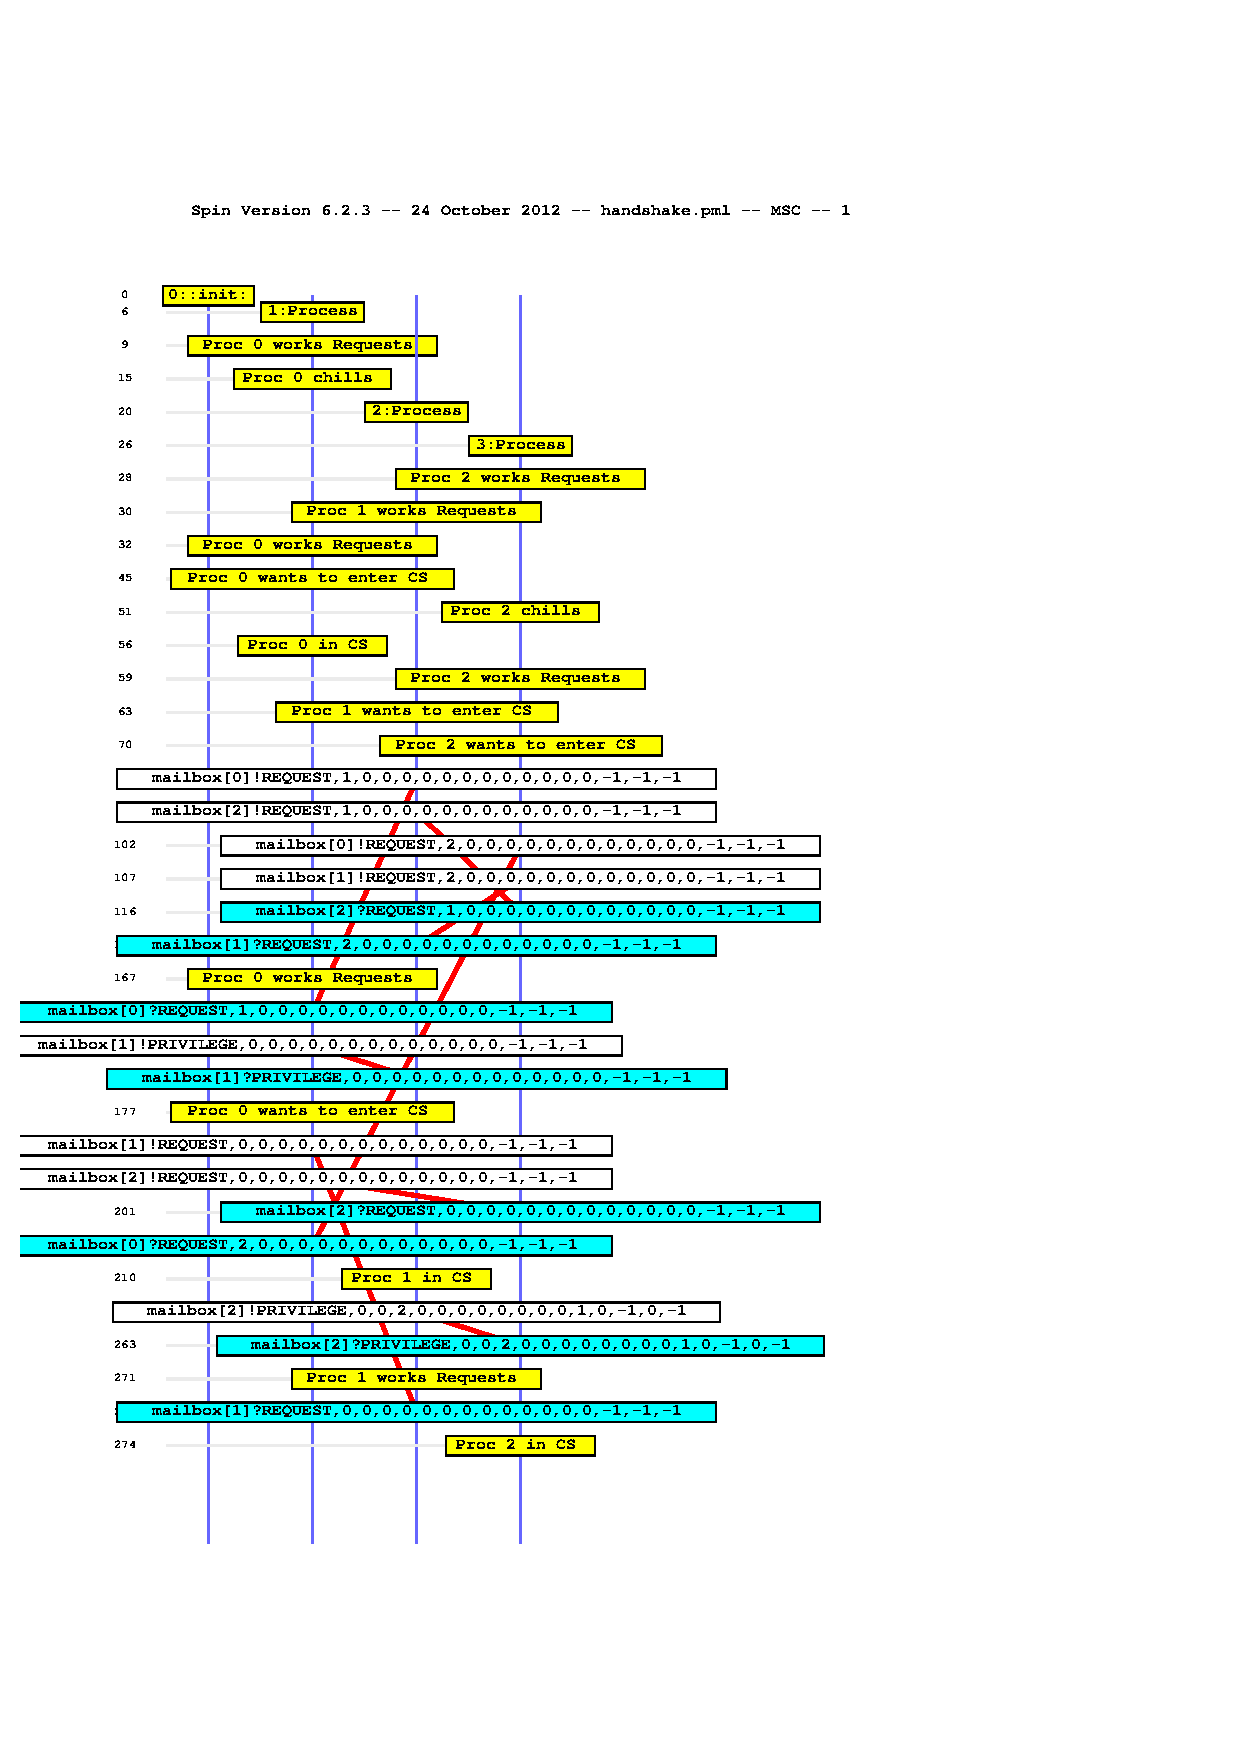
\includepdf[scale=0.8]{output/handshakesim.pdf}

%% --------------------------------------
%%           Section IV
%% --------------------------------------
\section{LTL Properties}

A Mutual Exclusion Algorithm needs to satisfy the four properties
\begin{itemize}
    \item Mutual Exclusion,
    \item Absence of Starvation,
    \item Fairness,
    \item No Unneccessary Delay
\end{itemize}
to be considered as correct.

In Spin we have to model for each of these properties one or more
LTL - Properties.

\subsection{Mutual Exclusion}

We added a variable \lstinline|incs| that is incremented before the critical section
and decremented aftarwards. If initialized to zero mutual exclusion is expressed by the
property
\begin{equation}
    \square \left( \text{\lstinline|incs|} \leq 1 \right)
\end{equation}
which is used in both implementations.

\subsection{Absence of Starvation}

For this property we need a label \lstinline|request|. We already have an array to keep track of the request,
but this flag is shortly after the critical section still set to one.
Using the counter \lstinline|incs| from the Mutual Exclusion property we can express deadlock freedom by
\begin{equation}
    \square \left( \left( \underset{0\leq i < N}{\bigvee} \text{\lstinline|Process[p[i]]@request|}\right) \Rightarrow \diamond \text{\lstinline|incs|} = 1 \right)
\end{equation}
again for both algorithms.
\subsection{Fairness}

All processes do not differ except for their Identifier. Therefore we will check the fairness constraint for the first process and the second process.
The first one because it has initially the privilage and the second one as a representive for every other process.
This time we used a label at the critical section and an array for the process id's.

Fairness can be expressed by
\begin{eqnarray}
    \square & ( \text{\lstinline|Process[p[0]]@request|} \Rightarrow \diamond \text{\lstinline|Process[p[0]]@critical|} \\
    &\land \text{\lstinline|Process[p[1]]@request|}\Rightarrow \diamond \text{\lstinline|Process[p[1]]@critical|})
\end{eqnarray}
in both algorithms.

\subsection{No Uneccessary Delay}

If we checked the previous property we have already a solution for this property.
This is because it holds that each process that wants to enter the cirtical section will do so eventually for each path in
the transition system.
If we want to check the property -- if a process wants to enter the critical section and other process arrives at the request section,
the first one will eventually enter the critical section -- this is only describes a subset of the paths considered in the fairness property.
Therefore if we have proofen that one, we have a proof for this one.

%% --------------------------------------
%%           Section V
%% --------------------------------------
\section{Checking the Properties}

We could see that the first algorithm has unbounded character. We let the verifier run for some time
and never saw an error (see APPENDIX).

\subsection{Unbounded Variant}

In this section we checked the first, unbounded variant of the algorithm.
Because it is unbounded the checking will never end. We therefore checked until we reached
a certain depth in the search tree and ended it afterwards.

\subsubsection{Mutual Exclusion}

We used the above described LTL property
\begin{lstlisting}
ltl claim1 { [] (incs <= 1)}
\end{lstlisting}
and run the verifier via
\begin{lstlisting}
gcc -DVECTORSZ=4096 -DCOLLAPSE pan.c -o pan
./pan -a
\end{lstlisting}

The verifier gave the output
\begin{lstlisting}
State-vector 2072 byte, depth reached 9999, errors: 0
 40921117 states, stored
 37895505 states, matched
 78816622 transitions (= stored+matched)
 56986035 atomic steps
hash conflicts:  29156326 (resolved)
\end{lstlisting}
which at least shows, that until this depth there was no error.
The full output can be see in \ref{mc:app:unb:mutex}.

\subsubsection{Absence of Starvation}

We used the LTL property
\begin{lstlisting}
ltl claim2 {[]((Process[p[0]]@request
||Process[p[1]]@request||Process[p[2]]@request)-><>(incs==1))}
\end{lstlisting}
and run the verifier via
\begin{lstlisting}
gcc -DVECTORSZ=4096 -DCOLLAPSE pan.c -o pan
./pan -a -f.
\end{lstlisting}
This time we need the parameter '-f'. Otherwise it is possible for one process to never to something after wanting to enter
the critical section. The output can be seen in \ref{mc:app:unb:dead} and it assures us that there is no error in
the searched depth.

\subsubsection{Fariness}

Here we checked the two claims

\begin{lstlisting}
ltl claim3 {[]( Process[p[0]]@request 
    -> <> (Process[p[0]]@cs))}
ltl claim4 {[]( Process[p[0]]@request 
    -> <> (Process[p[1]]@cs))}
\end{lstlisting}

which both could not be proven wrong after the execution of the verifier as in the last section.
The output can be seen in \ref{mc:app:unb:fair}.

\subsection{Bounded Variant}

This algorithm has a bounded state space and can be fully checked.
But we found an error in the property BLUBELIBLUBBLUB


\subsubsection{Absence of Starvation}

The second algorithm cannot be correct as proposed in the paper.
We have executed the algorithm several times and always reached a state in which
could no longer be made any progress. Because with a lifeness property we could
not perform a BFS to this event, we constructed the error from the error traces we saw.

Consider three processes p1, p2, p3 where p1 initially holds the privilege.
Now p1 and p2 enter the critical section swaping each round until both entered the critical section
L times. It holds that
$\text{RN}[0] =\text{RN}[1] = L - 1$ in both processes
and let be p1 be the process that aquired the priviledge last.\\

If p1 now leaves the critical section $\text{RN}[0] = L - 1$ holds and
p1 waits for two REPLAY messages which he will get because he has sended two REQUEST messages
while his requestCount was $L$. He receives those two messages and now atempts to
enter the critical section again. Because no other process wants to enter and he still holds
the priviledge he can do so.\\

On leaving the critical section again $\text{RN}[0] = L - 1$ holds because RN is only changed
if p1 does not have the priviledge. He now waits for two REPLY messages which he will never
receive because he never send REQUEST messages in the first place. Finally because he still
holds the priviledge no other process can enter the cirtical section and we reached a deadlock state.

\subsubsection{Fairness and No Unnecessary Delay}

If we have an algorithm that contains a Deadlock (Lifelock in this case) then neither 
Fairness nor `No Unnecessary Delay` can be satisfied because they both
depend on the fact that it is possible to enter the critical section.

\subsubsection{Mutual Exclusion}

We assume the algorithm satisfies at least mutual exclusion because in this matter it does not
differ from the first algorithm. But Spin couldn't check the property
because he could not perform the receive that led to the error mentioned afore.\\

Hence we could not check this property successful because Spin can not do so if a receive statement
runs into a deadlock state.

%% --------------------------------------
%%           Section VI
%% --------------------------------------
\section{Conclusion}

We modeled both algorithms of Suzuki and Kasami in promela. We were not able to verify either one of
both models to be correct. The first, of course, contains unbounded counters and thus cannot be 
fully checked. Nevertheless, we were able to show that for a certain search depth, the first algorithm does not contain any reachable errors. Here, we were able to show that the first algorithm is unlikely to contain
errors regarding safety and liveness properties.
However, the second algorithm did trigger a number of errors during model checking. The only property we could not refute is the safety property, yet we were again not able to perform an exhaustive state search. 
We are convinced that the second algorithm contains a deadlock and thus does not solve the mutual exclusion problem.

%% --------------------------------------
%%           Section ??
%% --------------------------------------
\addcontentsline{toc}{section}{References}
\bibliographystyle{splncs}

\bibliography{mc}

\chapter*{Appendix}
\begin{appendix}

\section{Unbonded Algorithm Output}

\subsection{Mutual Exclusion \label{mc:app:unb:mutex}}


\begin{lstlisting}[frame=single]

Alex@hildegunst ~
$ ./pan -a
error: max search depth too small
Depth=    9999 States=    1e+06 Transitions= 1.92e+06 Memory=   146.812 t=     7.21 R=   1e+05
Depth=    9999 States=    2e+06 Transitions= 3.83e+06 Memory=   228.453 t=     14.6 R=   1e+05
Depth=    9999 States=    3e+06 Transitions= 5.74e+06 Memory=   311.656 t=     22.4 R=   1e+05
Depth=    9999 States=    4e+06 Transitions= 7.68e+06 Memory=   402.281 t=     30.4 R=   1e+05
Depth=    9999 States=    5e+06 Transitions= 9.63e+06 Memory=   503.453 t=     38.3 R=   1e+05
Depth=    9999 States=    6e+06 Transitions= 1.16e+07 Memory=   582.750 t=     45.8 R=   1e+05
Depth=    9999 States=    7e+06 Transitions= 1.35e+07 Memory=   670.250 t=     53.1 R=   1e+05
Depth=    9999 States=    8e+06 Transitions= 1.54e+07 Memory=   744.859 t=     60.6 R=   1e+05
Depth=    9999 States=    9e+06 Transitions= 1.73e+07 Memory=   827.672 t=     68.3 R=   1e+05
Depth=    9999 States=    1e+07 Transitions= 1.93e+07 Memory=   914.000 t=     76.3 R=   1e+05
Depth=    9999 States=  1.1e+07 Transitions= 2.12e+07 Memory=   997.203 t=     83.9 R=   1e+05
Depth=    9999 States=  1.2e+07 Transitions= 2.31e+07 Memory=  1082.750 t=     91.5 R=   1e+05
Depth=    9999 States=  1.3e+07 Transitions= 2.51e+07 Memory=  1170.250 t=     99.2 R=   1e+05
Depth=    9999 States=  1.4e+07 Transitions=  2.7e+07 Memory=  1255.016 t=      107 R=   1e+05
Depth=    9999 States=  1.5e+07 Transitions=  2.9e+07 Memory=  1340.172 t=      115 R=   1e+05
Depth=    9999 States=  1.6e+07 Transitions= 3.09e+07 Memory=  1423.766 t=      123 R=   1e+05
Depth=    9999 States=  1.7e+07 Transitions= 3.28e+07 Memory=  1507.359 t=      131 R=   1e+05
Depth=    9999 States=  1.8e+07 Transitions= 3.47e+07 Memory=  1593.297 t=      139 R=   1e+05
Depth=    9999 States=  1.9e+07 Transitions= 3.67e+07 Memory=  1677.672 t=      146 R=   1e+05
Depth=    9999 States=    2e+07 Transitions= 3.86e+07 Memory=  1756.969 t=      154 R=   1e+05
Depth=    9999 States=  2.1e+07 Transitions= 4.05e+07 Memory=  1840.172 t=      162 R=   1e+05
Depth=    9999 States=  2.2e+07 Transitions= 4.25e+07 Memory=  1921.422 t=      170 R=   1e+05
Depth=    9999 States=  2.3e+07 Transitions= 4.44e+07 Memory=  2001.891 t=      178 R=   1e+05
Depth=    9999 States=  2.4e+07 Transitions= 4.63e+07 Memory=  2084.703 t=      186 R=   1e+05
Depth=    9999 States=  2.5e+07 Transitions= 4.83e+07 Memory=  2168.297 t=      194 R=   1e+05
Depth=    9999 States=  2.6e+07 Transitions= 5.02e+07 Memory=  2253.453 t=      202 R=   1e+05
Depth=    9999 States=  2.7e+07 Transitions= 5.21e+07 Memory=  2321.812 t=      210 R=   1e+05
Depth=    9999 States=  2.8e+07 Transitions=  5.4e+07 Memory=  2395.641 t=      218 R=   1e+05
Depth=    9999 States=  2.9e+07 Transitions= 5.59e+07 Memory=  2474.156 t=      226 R=   1e+05
Depth=    9999 States=    3e+07 Transitions= 5.79e+07 Memory=  2560.094 t=      234 R=   1e+05
Depth=    9999 States=  3.1e+07 Transitions= 5.98e+07 Memory=  2642.906 t=      242 R=   1e+05
Depth=    9999 States=  3.2e+07 Transitions= 6.17e+07 Memory=  2726.109 t=      251 R=   1e+05
Depth=    9999 States=  3.3e+07 Transitions= 6.36e+07 Memory=  2804.234 t=      259 R=   1e+05
Depth=    9999 States=  3.4e+07 Transitions= 6.55e+07 Memory=  2880.797 t=      267 R=   1e+05
pan: resizing hashtable to -w26..  done
Depth=    9999 States=  3.5e+07 Transitions= 6.74e+07 Memory=  3211.406 t=      282 R=   1e+05
Depth=    9999 States=  3.6e+07 Transitions= 6.94e+07 Memory=  3302.031 t=      290 R=   1e+05
Depth=    9999 States=  3.7e+07 Transitions= 7.13e+07 Memory=  3382.500 t=      298 R=   1e+05
tate-vector 2072 byte, depth reached 9999, errors: 0
 40921117 states, stored
 37895505 states, matched
 78816622 transitions (= stored+matched)
 56986035 atomic steps
hash conflicts:  29156326 (resolved)State-vector 2072 byte, 
    depth reached 9999, errors: 0
 40921117 states, stored
 37895505 states, matched
 78816622 transitions (= stored+matched)
 56986035 atomic steps
hash conflicts:  29156326 (resolved)
Depth=    9999 States=  3.9e+07 Transitions= 7.51e+07 Memory=  3546.172 t=      314 R=   1e+05
Depth=    9999 States=    4e+07 Transitions= 7.71e+07 Memory=  3636.016 t=      322 R=   1e+05
pan: out of memory

hint: to reduce memory, recompile with
  -DMA=2072   # better/slower compression, or
  -DBITSTATE # supertrace, approximation

(Spin Version 6.2.3 -- 24 October 2012)
Warning: Search not completed
        + Partial Order Reduction
        + Compression

Full statespace search for:
        never claim             + (claim1)
        assertion violations    + (if within scope of claim)
        acceptance   cycles     + (fairness disabled)
        invalid end states      - (disabled by never claim)

State-vector 2072 byte, depth reached 9999, errors: 0
 40921117 states, stored
 37895505 states, matched
 78816622 transitions (= stored+matched)
 56986035 atomic steps
hash conflicts:  29156326 (resolved)

Stats on memory usage (in Megabytes):
81641.175       equivalent memory usage for states 
    (stored*(State-vector + overhead))
 3442.784       actual memory usage for states (compression: 4.22%)
                state-vector as stored = 68 byte + 20 byte overhead
  256.000       memory used for hash table (-w26)
    0.382       memory used for DFS stack (-m10000)
    1.840       memory lost to fragmentation
 3697.344       total actual memory usage


nr of templates: [ 0:globals 1:chans 2:procs ]
collapse counts: [ 0:4015087 2:13 3:3852 4:1 ]

pan: elapsed time 329 seconds
pan: rate 124449.14 states/second
\end{lstlisting}

\subsubsection{Absence of Starvation}
\label{mc:app:unb:dead}

\begin{lstlisting}[frame=single]

Alex@hildegunst ~
$ gcc -DVECTORSZ=4096 -DCOLLAPSE pan.c -o pan

Alex@hildegunst ~
$ ./pan -a -f
error: max search depth too small
Depth=    9999 States=    1e+06 Transitions= 2.55e+06 Memory=    95.250 t=     10.2 R=   1e+05
Depth=    9999 States=    2e+06 Transitions= 4.91e+06 Memory=   120.641 t=     19.2 R=   1e+05
Depth=    9999 States=    3e+06 Transitions= 7.25e+06 Memory=   145.250 t=     28.3 R=   1e+05
Depth=    9999 States=    4e+06 Transitions= 9.61e+06 Memory=   166.344 t=     37.5 R=   1e+05
Depth=    9999 States=    5e+06 Transitions=  1.2e+07 Memory=   194.859 t=     47.5 R=   1e+05
Depth=    9999 States=    6e+06 Transitions= 1.43e+07 Memory=   222.203 t=     57.8 R=   1e+05
Depth=    9999 States=    7e+06 Transitions= 1.67e+07 Memory=   246.031 t=     66.6 R=   1e+05
Depth=    9999 States=    8e+06 Transitions=  1.9e+07 Memory=   268.297 t=     75.6 R=   1e+05
Depth=    9999 States=    9e+06 Transitions= 2.13e+07 Memory=   289.000 t=     84.1 R=   1e+05
Depth=    9999 States=    1e+07 Transitions= 2.36e+07 Memory=   313.219 t=     93.6 R=   1e+05
Depth=    9999 States=  1.1e+07 Transitions=  2.6e+07 Memory=   333.141 t=      103 R=   1e+05
Depth=    9999 States=  1.2e+07 Transitions= 2.83e+07 Memory=   358.531 t=      113 R=   1e+05
Depth=    9999 States=  1.3e+07 Transitions= 3.08e+07 Memory=   383.141 t=      123 R=   1e+05
Depth=    9999 States=  1.4e+07 Transitions= 3.31e+07 Memory=   407.359 t=      131 R=   1e+05
Depth=    9999 States=  1.5e+07 Transitions= 3.54e+07 Memory=   430.406 t=      140 R=   1e+05
Depth=    9999 States=  1.6e+07 Transitions= 3.77e+07 Memory=   453.453 t=      149 R=   1e+05
Depth=    9999 States=  1.7e+07 Transitions=    4e+07 Memory=   476.500 t=      158 R=   1e+05
Depth=    9999 States=  1.8e+07 Transitions= 4.24e+07 Memory=   497.984 t=      168 R=   1e+05
Depth=    9999 States=  1.9e+07 Transitions= 4.48e+07 Memory=   520.641 t=      180 R=   1e+05
Depth=    9999 States=    2e+07 Transitions= 4.71e+07 Memory=   544.859 t=      189 R=   1e+05
Depth=    9999 States=  2.1e+07 Transitions= 4.94e+07 Memory=   568.688 t=      198 R=   1e+05
Depth=    9999 States=  2.2e+07 Transitions= 5.18e+07 Memory=   592.906 t=      207 R=   1e+05
Depth=    9999 States=  2.3e+07 Transitions=  5.4e+07 Memory=   615.172 t=      215 R=   1e+05
Depth=    9999 States=  2.4e+07 Transitions= 5.64e+07 Memory=   640.172 t=      225 R=   1e+05
Depth=    9999 States=  2.5e+07 Transitions= 5.88e+07 Memory=   658.922 t=      235 R=   1e+05
Depth=    9999 States=  2.6e+07 Transitions= 6.11e+07 Memory=   681.969 t=      243 R=   1e+05
Depth=    9999 States=  2.7e+07 Transitions= 6.34e+07 Memory=   704.234 t=      252 R=   1e+05
Depth=    9999 States=  2.8e+07 Transitions= 6.58e+07 Memory=   730.406 t=      263 R=   1e+05
Depth=    9999 States=  2.9e+07 Transitions= 6.81e+07 Memory=   752.281 t=      272 R=   1e+05
Depth=    9999 States=    3e+07 Transitions= 7.05e+07 Memory=   775.328 t=      281 R=   1e+05
Depth=    9999 States=  3.1e+07 Transitions= 7.28e+07 Memory=   795.641 t=      290 R=   1e+05
Depth=    9999 States=  3.2e+07 Transitions= 7.51e+07 Memory=   817.125 t=      299 R=   1e+05
Depth=    9999 States=  3.3e+07 Transitions= 7.74e+07 Memory=   837.438 t=      309 R=   1e+05
Depth=    9999 States=  3.4e+07 Transitions= 7.97e+07 Memory=   861.656 t=      318 R=   1e+05
pan: resizing hashtable to -w26..  done
Depth=    9999 States=  3.5e+07 Transitions= 8.21e+07 Memory=  1125.859 t=      329 R=   1e+05
Depth=    9999 States=  3.6e+07 Transitions= 8.44e+07 Memory=  1150.859 t=      339 R=   1e+05
Depth=    9999 States=  3.7e+07 Transitions= 8.67e+07 Memory=  1168.047 t=      348 R=   1e+05
Depth=    9999 States=  3.8e+07 Transitions=  8.9e+07 Memory=  1189.531 t=      358 R=   1e+05
.....

Depth=    9999 States= 1.46e+08 Transitions= 3.43e+08 Memory=  3616.094 t= 1.41e+03 R=   1e+05
Depth=    9999 States= 1.47e+08 Transitions= 3.45e+08 Memory=  3641.094 t= 1.42e+03 R=   1e+05
Depth=    9999 States= 1.48e+08 Transitions= 3.47e+08 Memory=  3663.359 t= 1.43e+03 R=   1e+05
Depth=    9999 States= 1.49e+08 Transitions=  3.5e+08 Memory=  3683.281 t= 1.44e+03 R=   1e+05
pan: out of memory
hint: to reduce memory, recompile with
  -DMA=2084   # better/slower compression, or
  -DBITSTATE # supertrace, approximation

(Spin Version 6.2.3 -- 24 October 2012)
Warning: Search not completed
        + Partial Order Reduction
        + Compression

Full statespace search for:
        never claim             + (claim2)
        assertion violations    + (if within scope of claim)
        acceptance   cycles     + (fairness enabled)
        invalid end states      - (disabled by never claim)

State-vector 2084 byte, depth reached 9999, errors: 0
 51599459 states, stored (1.49533e+08 visited)
2.0147333e+08 states, matched
3.5100596e+08 transitions (= visited+matched)
3.592431e+08 atomic steps
hash conflicts:  41393391 (resolved)

Stats on memory usage (in Megabytes):
103535.902      equivalent memory usage for states 
    (stored*(State-vector + overhead))
 3441.959       actual memory usage for states (compression: 3.32%)
                state-vector as stored = 50 byte + 20 byte overhead
  256.000       memory used for hash table (-w26)
    0.382       memory used for DFS stack (-m10000)
    1.403       memory lost to fragmentation
 3696.953       total actual memory usage


nr of templates: [ 0:globals 1:chans 2:procs ]
collapse counts: [ 0:3040490 2:13 3:3918 4:2 ]

pan: elapsed time 1.44e+03 seconds
pan: rate 103649.56 states/second
\end{lstlisting}

\subsection{Fairness}
\label{mc:app:unb:fair}

\begin{lstlisting}[frame=single]

Alex@hildegunst ~
$ gcc -DVECTORSZ=4096 -DCOLLAPSE -DMEMLIM=2048 pan.c -o pan

Alex@hildegunst ~
$ ./pan -a -f
Depth=    9999 States=    1e+06 Transitions= 2.51e+06 Memory=    87.828 t=     9.83 R=   1e+05
Depth=    9999 States=    2e+06 Transitions= 4.96e+06 Memory=   108.922 t=     19.4 R=   1e+05
Depth=    9999 States=    3e+06 Transitions= 7.48e+06 Memory=   129.625 t=     29.5 R=   1e+05
Depth=    9999 States=    4e+06 Transitions= 9.92e+06 Memory=   150.328 t=       39 R=   1e+05
Depth=    9999 States=    5e+06 Transitions= 1.24e+07 Memory=   172.984 t=       49 R=   1e+05
Depth=    9999 States=    6e+06 Transitions= 1.49e+07 Memory=   197.594 t=     59.8 R=   1e+05
Depth=    9999 States=    7e+06 Transitions= 1.75e+07 Memory=   221.031 t=     71.3 R=   1e+05
Depth=    9999 States=    8e+06 Transitions= 2.01e+07 Memory=   243.688 t=     81.6 R=   1e+05
Depth=    9999 States=    9e+06 Transitions= 2.26e+07 Memory=   266.734 t=     91.8 R=   1e+05
Depth=    9999 States=    1e+07 Transitions= 2.51e+07 Memory=   288.609 t=      101 R=   1e+05
Depth=    9999 States=  1.1e+07 Transitions= 2.76e+07 Memory=   308.922 t=      112 R=   1e+05
Depth=    9999 States=  1.2e+07 Transitions= 3.01e+07 Memory=   332.359 t=      121 R=   1e+05
Depth=    9999 States=  1.3e+07 Transitions= 3.26e+07 Memory=   354.234 t=      131 R=   1e+05
Depth=    9999 States=  1.4e+07 Transitions= 3.51e+07 Memory=   377.672 t=      141 R=   1e+05
Depth=    9999 States=  1.5e+07 Transitions= 3.76e+07 Memory=   402.672 t=      152 R=   1e+05
Depth=    9999 States=  1.6e+07 Transitions=    4e+07 Memory=   423.766 t=      161 R=   1e+05
Depth=    9999 States=  1.7e+07 Transitions= 4.26e+07 Memory=   444.469 t=      171 R=   1e+05
Depth=    9999 States=  1.8e+07 Transitions= 4.51e+07 Memory=   465.172 t=      181 R=   1e+05
Depth=    9999 States=  1.9e+07 Transitions= 4.77e+07 Memory=   485.484 t=      192 R=   1e+05
Depth=    9999 States=    2e+07 Transitions= 5.02e+07 Memory=   511.266 t=      203 R=   1e+05
Depth=    9999 States=  2.1e+07 Transitions= 5.27e+07 Memory=   532.750 t=      213 R=   1e+05
Depth=    9999 States=  2.2e+07 Transitions= 5.52e+07 Memory=   554.234 t=      223 R=   1e+05
Depth=    9999 States=  2.3e+07 Transitions= 5.78e+07 Memory=   572.594 t=      233 R=   1e+05
Depth=    9999 States=  2.4e+07 Transitions= 6.03e+07 Memory=   588.219 t=      244 R=   1e+05
Depth=    9999 States=  2.5e+07 Transitions= 6.27e+07 Memory=   607.750 t=      253 R=   1e+05
Depth=    9999 States=  2.6e+07 Transitions= 6.52e+07 Memory=   630.406 t=      264 R=   1e+05
Depth=    9999 States=  2.7e+07 Transitions= 6.77e+07 Memory=   651.109 t=      273 R=   1e+05
Depth=    9999 States=  2.8e+07 Transitions= 7.02e+07 Memory=   672.594 t=      284 R=   1e+05
Depth=    9999 States=  2.9e+07 Transitions= 7.27e+07 Memory=   694.078 t=      295 R=   1e+05
Depth=    9999 States=    3e+07 Transitions= 7.52e+07 Memory=   717.125 t=      306 R=   1e+05
Depth=    9999 States=  3.1e+07 Transitions= 7.76e+07 Memory=   736.656 t=      315 R=   1e+05
Depth=    9999 States=  3.2e+07 Transitions= 8.01e+07 Memory=   756.578 t=      326 R=   1e+05
Depth=    9999 States=  3.3e+07 Transitions= 8.26e+07 Memory=   776.891 t=      336 R=   1e+05
Depth=    9999 States=  3.4e+07 Transitions= 8.52e+07 Memory=   799.547 t=      347 R=   1e+05
pan: resizing hashtable to -w26..  done
Depth=    9999 States=  3.5e+07 Transitions= 8.78e+07 Memory=  1058.281 t=      360 R=   1e+05
....
Depth=    9999 States=  1.1e+08 Transitions= 2.75e+08 Memory=  2727.812 t= 1.17e+03 R=   9e+04
Interrupted

(Spin Version 6.2.3 -- 24 October 2012)
Warning: Search not completed
        + Partial Order Reduction
        + Compression

Full statespace search for:
        never claim             + (claim3)
        assertion violations    + (if within scope of claim)
        acceptance   cycles     + (fairness enabled)
        invalid end states      - (disabled by never claim)

State-vector 2084 byte, depth reached 9999, errors: 0
 35000887 states, stored (1.10849e+08 visited)
1.6674613e+08 states, matched
2.7759498e+08 transitions (= visited+matched)
2.8812403e+08 atomic steps
hash conflicts:  22501231 (resolved)

Stats on memory usage (in Megabytes):
70230.356       equivalent memory usage for states 
    (stored*(State-vector + overhead))
 2492.384       actual memory usage for states (compression: 3.55%)
                state-vector as stored = 55 byte + 20 byte overhead
  256.000       memory used for hash table (-w26)
    0.382       memory used for DFS stack (-m10000)
    1.435       memory lost to fragmentation
 2747.344       total actual memory usage


nr of templates: [ 0:globals 1:chans 2:procs ]
collapse counts: [ 0:2257676 2:13 3:4776 4:2 ]

pan: elapsed time 1.18e+03 seconds
pan: rate 93661.735 states/second
\end{lstlisting}
\end{appendix}
\end{document}
